\chapter{Player behavior modeling}\label{ch:modeling}

Having identified an activity recognition system, we aimed at the definition of an approach to model user behavior that could account for the combination of the player physical effort and interaction level. The proposed model is based on the human activity recognition (chapter~\ref{ch:activity}) and a description of interaction (proximity and body contraction index) relative to the robot co-player.
%ANDY If you have described separately the activity recognition model based on the accelerometer, a separate chapter has to be dedicated also to the lasers or whatever you would like to consider for the other parameters.  All these sources are functional to provide data for the activity model (if you like you may have all the contributions in the same chapter).

\section{Relational Activity Model}\label{sec:simple_model}

As in~\cite{etheredge_generic_2013}, we defined as behavior a sequence of discrete time-bounded actions performed by the player. Since we are dealing with a physically interactive scenario, these time-bounded actions have strong relation with the amount of physical activity spent, hereby considered as the human ``activity effort''. The relationship with the robot, on the other hand, is considered the ``relative interaction''. 

In the proposed model, the two dimensions (activity and interaction) are combined into a simple overall scoring system capable of describing quantitatively the player's active participation in the~\gls{pirg}. The proposed model is detailed in the next.

\subsection{Activity}\label{activity}

Equation~\ref{eq:activity_eq} is used to compute the general amount of activity $\alpha(m)$, given the classification of primitive motions from chapter~\ref{ch:activity}:

\begin{equation}
	\alpha(m)=\sum_{i \in \mathcal{A}} \omega_{i}\varphi_i(m);\qquad m \in \mathcal{M}
	\label{eq:activity_eq}
\end{equation}
, where $\mathcal{A}$ stands for the set of activities \{``running'', ``locally moving'', ``walking/dodging''\}; $\omega$ stands for the activity weight; $\varphi$ for the stochastic prediction value for the motion primitive $m$.

We consider equation~\ref{eq:activity_eq} as a measure of the ``effort'' of the player. The weight $\omega$ states how much each physical activity contributes to the overall quantification and is a hyper-parameter intended to capture the partial ordering among activities.

\subsection{Interaction}\label{Interaction}
In order to model the interaction we take into account the spatial relationship between the player and the robot defined as \textit{proximity} and a measure of body contraction named~\gls{ci}.

Proximity is a measure defined in the interval [0, 1], computed from the data provided by the Microsoft Kinect\textsuperscript{\textregistered}, normalized given the sensor specifications (see section~\ref{sec:kinectsec}).~\gls{ci} is also in [0, 1] and it is calculated using a technique related to the bounding region, i.e., the minimum rectangle surrounding the body: the algorithm compares the area covered by this rectangle with the area currently covered by the player's silhouette~\citep{castellano_recognising_2007}.

A high~\gls{ci} is associated with an intense interaction because a wide openness of the body is interpreted as a higher focus level of the player w.r.t the robot and to the game; for this reason it will boost the final outcome. Low~\gls{ci}, in turn, is interpreted as a lack of focus or, in general, limited motivation of the player, which penalizes the interaction.%ANDY: Not providing data and analysis to support this makes this assumption quite weak.

\subsection{Combined model}\label{sec:engagement}
The model to describe the player's relational activity is a combination of the activity level and the degree of interaction, named $\epsilon$; it summarizes the player physical activity during the game and has a linear relationship with his interaction with the robotic opponent as follows: 
\begin{equation}
\label{enagementeq}
\epsilon=\kappa + \alpha(m),
\end{equation}

where $\kappa= (1-\rho)c$.  The $c$ in the calculation of $\kappa$ represents a constant whose function is just that of change the numerical range of the variable and is assumed greater than zero. $\kappa$ also uses the degree of interaction $\rho$ so that when the estimated interaction is zero (meaning no interaction) the activity level is only $\alpha$. In other words, $\kappa$ is the a term whose function is to boosts the importance of the activity by putting it in relation with the amount of interaction. 

Notice, however, that $\rho$ is an overall degree of interaction, i.e., the combination of~\gls{ci} and proximity. The exact procedure for the combination of the interaction signals is not bound to a specific method. In this work, we have used a fuzzy logic system to obtain the desired combination, described in a linguistic way. In principle, the combination of the signals depends on the specifics of the~\gls{pirg} environment.

For the evaluation of the model we have reused the same data from section~\ref{sec:data_collection}. The model output for two different players can be seen in Figure~\ref{fig:model_output}. In Figure~\ref{fig:fun}, the player is perceived as more active than the one in fig.~\ref{fig:nofun}, which is reflected by the difference in the inactivity time and the amplitude of the bars.

\begin{figure}[h]
    \centering 
	\begin{subfigure}[h]{5cm}
		\centering      
		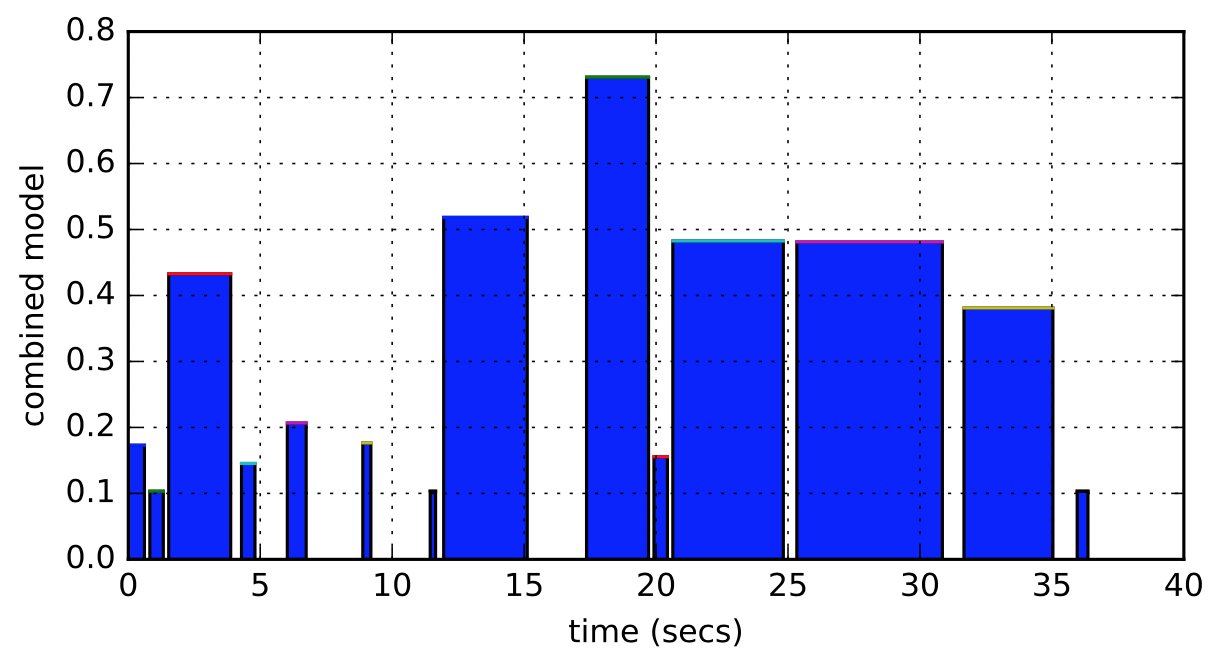
\includegraphics[draft=false, width=5cm]{images/04-activity/combined.png}
		\caption{}
		\label{fig:fun}
	\end{subfigure}
	~
	\begin{subfigure}[h]{5cm}
		\centering      
      	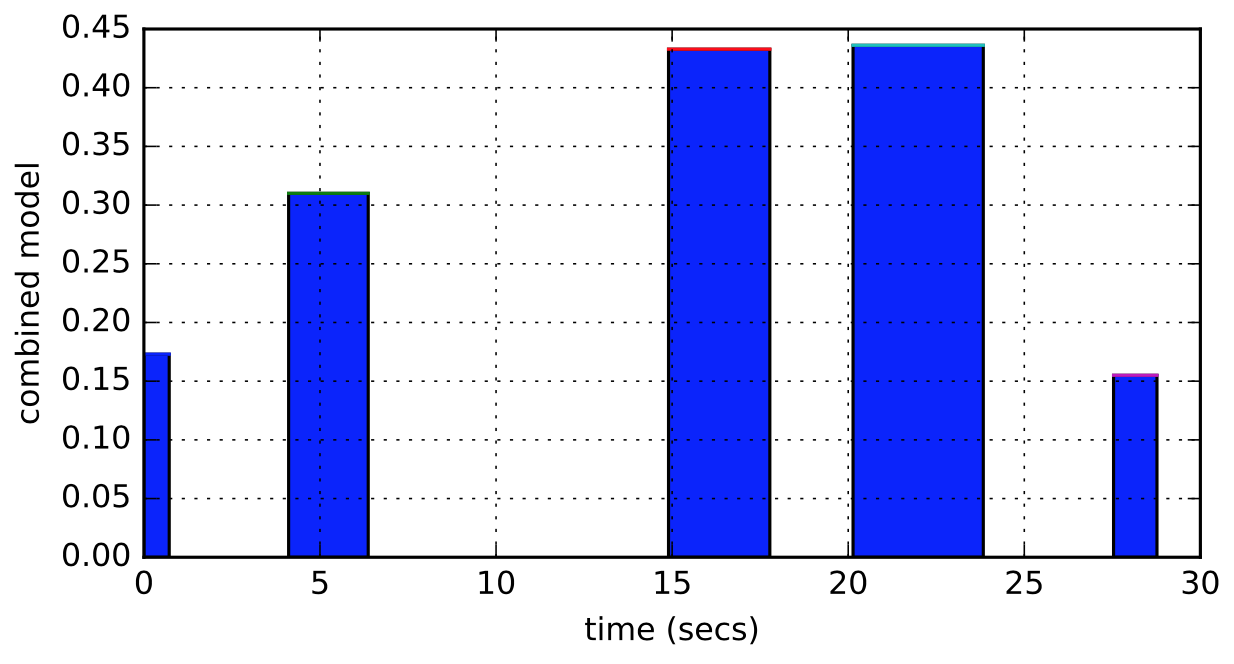
\includegraphics[draft=false,width=5cm]{images/04-activity/combined_less.png}
      	\caption{}
      	\label{fig:nofun}
     \end{subfigure}
      \caption{a) Model results for a single match that lasted 45 secs. b) Model output for a less active player. The graph refers to 30 initial secs of activity.}		
      \label{fig:model_output}
\end{figure}

The model quantitatively describe, in a simple way, the player's relational activity by the combination of the amount of physical activity and interaction relative to the robot. This can be used as a metric expected to enable the robot to take into account the player's attitude in order to adapt its own activity to match it. Using this model, for instance, an active player could be viewed as one having a larger cumulative sum of $\epsilon$ values up to a point in time.

However, this model is limited in several ways, %ANDY I cannot evaluate it since I cannot understand it
one of which is the manual definition of weights for the activities ($\omega$). Manually selecting these scaling factors becomes difficult as the number of activities grows. With this in mind, we have then worked on a definition of a more robust player model relying on latent representation which  is describe next.

\section{Latent player modeling}

We attempted to improve upon the previous model in several ways. First, by mapping the stream of accelerometer data to an image representation, called Gramian Angular Field (GAF) images~\citep{wang_imaging_2015}. We do this in order to take advantage from algorithms for unsupervised feature extraction, such as autoencoders~\citep{goodfellow_deep_2016}, and reduce the effort in handcrafting representation features for the user behavior. After the definition of a dictionary of primitives on the feature space, we apply ~\gls{lda}~\citep{blei_latent_2003}, a discrete generative model (an admixture model) mostly used for document retrieval and classification, to uncover coherent groups of motion patterns that can be used to categorize players.

The model here is comprehensively different from the simple one presented in the previous section: it does not take into account features of interaction, but only the player's acceleration patterns (despite not being considered, there is no fundamental constraint from which to prevent the use of such data); there is also no need to manually set scaling factors from target activities since the model explores the importance of each acceleration spike by itself; furthermore, the model is able to provide on its own the distinction between players so that it can easily be used for clustering. Each player is player is represented by a normalized vector where each component denotes the proportion of membership for a given class of players uncovered from data.

In special, our decision to use~\gls{lda} was inspired by the work of~\cite{smith_mining_2016}, which considers each game session as a ``document'' and the player generated stream data as the ``words'' of such document. The interpretation of game session as documents and player data as words preserves the jargon of the text mining and information retrieval literature from which~\gls{lda} is most used for. The main assumption is that different players generate different streams of input words, thus different  ``documents'', depending on their own motivation or play style. 

The feasibility of applying~\gls{lda} to this problem is further reinforced by noticing the apparent difficulty in objectively separating the existing types of motion patterns in the acceleration signal via inspection. A player in his/her playing activity may show different motion patterns that are often not clearly distinguishable between each other and thus not easy to provide a supervision for,~\ie a class tag. Here, the assumption is that a high motion profile, i.e., high turbulence in acceleration signal, is typical for a highly motivated player, since we believe a non-motivated player tends to stay relatively still, or to show a very low acceleration profile.

The claim that motion patterns convey engagement or even emotional state~\citep{aristidou_emotion_2015,shafir_emotion_2016,tsachor_somatic_2017} has been supported by several academic papers. Systematic approaches for describing body movement, such as~\gls{lma}~\citep{laban_language_1974}, are often used to derive low-dimensional representation of mood, facilitating affective motion modeling~\citep{burton_laban_2016}. This same type of analysis has been applied when investigating motor elements that characterize movements whose execution enhances basic emotions, such as: anger, fear, happiness and sadness~\citep{shafir_emotion_2016}. In game situations, despite the limited capacity for entertainment detection and modeling in Exergames, \gls{lma} had been reported as useful in fostering emotion recognition in states like: concentration, meditation, excitement and frustration~\citep{zacharatos_emotion_2013}.

Here, we hypothesize that, on average, a player will display his/her game-intrinsic motion style and convey some information about his/her interest in/motivation to play. Discovering which coherent groups of motion style exist in a dataset allows us to estimate to what extent an unknown player relates in terms of his/her own motion profile to known groups. This may ultimately support the design of~\gls{pirg}s able to adapt in order to offer a better play experience.

In summary, in our methodology a player is represented by how much of each discovered motion groups (called motion \textit{topics}) his/her data is likely to be generated from. Such representation is called the player's \textit{mixture proportion} of motion types and is akin to the mixture proportion of documents in topic modeling applications~\citep{blei_latent_2003}. We expect to see similar players grouped together in a coherent collection, enabling to distinguish among them and their motion types. The results obtained using the dataset detailed in section~\ref{sec:data_collection} are validated with human supervision, suggesting the applicability of our method to future mechanisms for designing auto-adapting agents.

\subsection{Problem Statement}
This section formulates the problem of modeling the player as a probabilistic mixture of player styles derived from data. One can see that it is a step towards advancements in the dimension of design referred to the ability to play for engagement maximization, as discussed in section~\ref{sec:dimensions}.

Here, we use data coming from a single accelerometer placed on the human player's body as in Chapter~\ref{ch:activity}; For the current study, player movement is our primary source of information for characterizing the playing style. The basic assumption is that a highly active player would naturally express his/her status by a very turbulent motion signal, making the signal compatible with strong in-game activity. Consider, for instance, the difference in signal shapes reported in Figure~\ref{figure:acc_signal_shape}.

\begin{figure}[h]
    \centering
    \begin{subfigure}[h]{\textwidth}
        \centering
        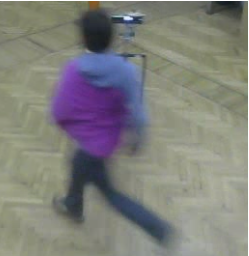
\includegraphics[width=0.2\textwidth]{images/05-modeling/enricorun.png} 
        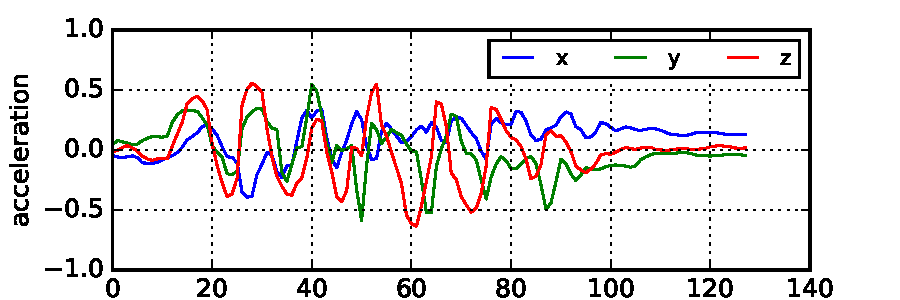
\includegraphics[width=0.6\textwidth]{images/05-modeling/running_sig_profile.eps} 
        \caption{}
    \end{subfigure}\vspace{6pt}
    ~
    \begin{subfigure}[h]{\textwidth}
        \centering
        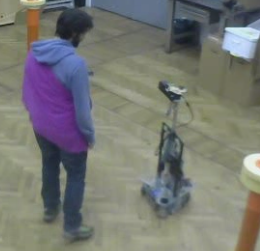
\includegraphics[width=0.2\textwidth]{images/05-modeling/enricostill.png}
        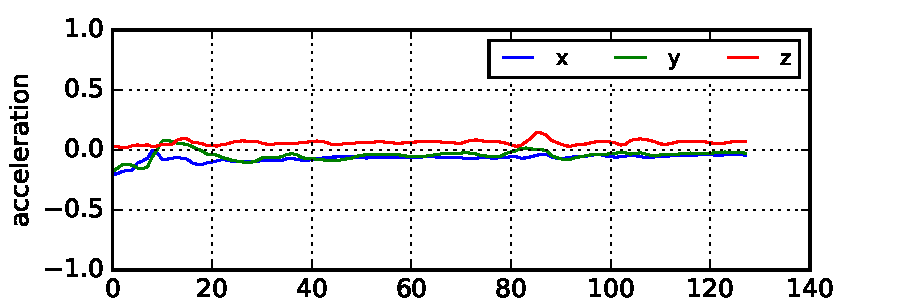
\includegraphics[width=0.6\textwidth]{images/05-modeling/standing_sig_profile.eps} 
        \caption{}
    \end{subfigure} \vspace{-6pt}
    \caption{Three-axis accelerometer signal during game play. a) A running player. b) A player standing still. Signal shape and amplitude are very characteristic for the respective activity.}
    \label{figure:acc_signal_shape}
\end{figure} \unskip

In other words, following this line of reasoning, we also assume players do not fake their engagement by unnecessarily performing strong activities, like running, when they are actually not engaged in the game or feel bored by the robot behavior. Therefore, we assume that a highly motivated player would act more intensively and frequently than a non-motivated one, thus showing a more turbulent acceleration signal profile. In situations like~\gls{pirg}, movement information is useful and should not be disregarded. Furthermore, a model that is able to extract a description of the player's movement profile for the purpose of robot behavior adaptation would generate interesting insights on the capability of the application to engage humans.

\subsection{Mathematical background}
This section presents the basic concepts and principles behind~\gls{gaf}, autoencoders and~\gls{lda}, which are important to understand our modeling procedure.

\subsubsection{\glsdesc{gaf} Images}

The results obtained in this work rely on the transformation of the acceleration time series generated by the player into images that are then processed and understood in terms of emergent patterns. The types of image we have chosen are~\gls{gasf} and~\gls{gadf}. Such images had been proposed in the field of time series classification~\citep{wang_imaging_2015}, where the authors evaluated the efficacy of representing time series in a polar coordinate system instead of the typical Cartesian coordinates. For a deep understanding of the method, we suggest reading the work of~\cite{wang_imaging_2015} since the authors did not only present the idea of~\gls{gasf}/\gls{gadf}, but also reported experimental results comparing them with other time series techniques. Here, we present an overview of the idea behind the method in order to familiarize the reader and to point out its role in our proposal.

In general, in order to obtain a~\gls{gasf}/\gls{gadf} representation for a time series $\mathcal{X}=\{x_{1}, x_{2}, ... x_{n}\}$ of size $n \in \mathbb{N}_{>0}$, rescaling is first performed in order to put the time series in the interval $[\,-1,1] \,$ or $[\,0,1]\,$. The second step is to represent the rescaled time series $\widetilde{\mathcal{X}}$ in polar coordinates, where each sample value is now mapped into the angular cosine and the time stamp information is represented as the radius. 
The formula for this step is as follows:

\begin{equation}
\begin{dcases}
  \phi = \arccos(\widetilde{x}_{i}) \quad -1 \leq \widetilde{x}_{i} \leq 1, \widetilde{x}_{i} \in \widetilde{\mathcal{X}} \\
  r = \frac{t_{i}}{N} \quad \quad t_{i} \in \mathbb{N}_{>0},
\end{dcases}
\label{equation:GAF}
\end{equation} 
where $t_{i}$ is the time stamp and $N$ plays the role of a normalizer for the span of the polar coordinate system. Some properties of this transformation are known:

\begin{itemize}[leftmargin=*,labelsep=5.8mm]
\item \textbf{{Property \#1}}: equation~(\ref{equation:GAF}) is bijective as $\cos(\phi)$ is monotonic when $\phi \in [\,0,\pi]\,$. Given a time series, the proposed map produces a unique result in the polar coordinate system together with a unique inverse map. 
\item \textbf{{Property \#2}}: as opposed to Cartesian coordinates, polar coordinates preserve absolute temporal~relations.
\item \textbf{{Property \#3}}: rescaled data in different intervals have different angular bounds. That is, $[\,0,1]\,$ corresponds to the cosine function in $[\,0,\frac{\pi}{2}]\,$, while cosine values in the interval $[\,-1,1]\,$ fall into the angular bounds $[\,0,\pi]\,$. These intervals are known to produce different information granularity in the~\gls{gaf}, especially for classification tasks~\citep{wang_imaging_2015}.
\end{itemize}

The third step in completing the transformation is to exploit the angular perspective by considering the trigonometric sum/difference between each point. This allows for the identification of the temporal correlation within different time intervals. The two types of~\gls{gaf}, namely~\gls{gasf} and~\gls{gadf}, are obtained as follows:

\begin{equation}
\begin{aligned}
\gls{gasf} &= [\,\cos(\phi_{i} + \phi{j}]\, \\
	 &= \widetilde{\mathcal{X}}' \cdot \widetilde{\mathcal{X}} - \sqrt{I-\widetilde{\mathcal{X}}^2}' \cdot \sqrt{I-\widetilde{\mathcal{X}}^2}
\end{aligned}
\end{equation}
\\
\begin{equation}
\begin{aligned}
\gls{gadf} &= [\,\sin(\phi_{i} + \phi{j}]\, \\
	 &= \sqrt{I-\widetilde{\mathcal{X}}^2}' \cdot \widetilde{\mathcal{X}} - \widetilde{\mathcal{X}}' \cdot \sqrt{I-\widetilde{\mathcal{X}}^2}\\
\end{aligned}
\end{equation}

The symbol $I$ is the unit row vector. After translating the time series from the Cartesian to polar coordinate system, each time step in it is taken as a 1D metric space. By defining the inner product as $<x,y> = x \cdot y - \sqrt{1-x^2} \cdot \sqrt{1-y^2}$ and $<x,y> = \sqrt{1-x^2} \cdot y - x \cdot \sqrt{1-y^2}$,
respectively,~\gls{gaf}s become {quasi-Gramian} matrices, since the defined $<x,y>$ do not satisfy the property of linearity in inner-product space.

According to~\cite{wang_imaging_2015}, the~\gls{gaf}s have several advantages:

\begin{itemize}[leftmargin=*,labelsep=5.8mm]
\item \textbf{{Advantage \#1}}: they provide a way to preserve temporal information. The temporal correlation is present because $G_{(i,j||i-j|=k)}$ represents the relative correlation by the superposition/difference of directions with respect to time interval $k$. The main diagonal $G_{i,i}$ is the special case when $k = 0$, which contains the original value/angular information. 
\item \textbf{{Advantage \#2:}} from the main diagonal, it is possible to reconstruct the time series back into the original Cartesian space. This is useful especially in a classification task, where we can convert the time series back to numerical Cartesian space from the high level features learned by, for instance, a deep neural network.
\end{itemize}

However, the size of the Gramian matrix $G$ is $n \times n$, for $n$ being the length of the raw time series. Which may produce issues regarding memory complexity. For this issue~\cite{wang_imaging_2015} propose a solution by attempting to reduce the size of the produced~\gls{gaf} using, for instance,~\gls{paa}~\citep{keogh_scaling_2000} to smooth the time series while preserving the trends. An example of the conversion from time series to~\gls{gasf} image is shown in Figure~\ref{figure:gasf_example}.

\begin{figure} [h]
\centering
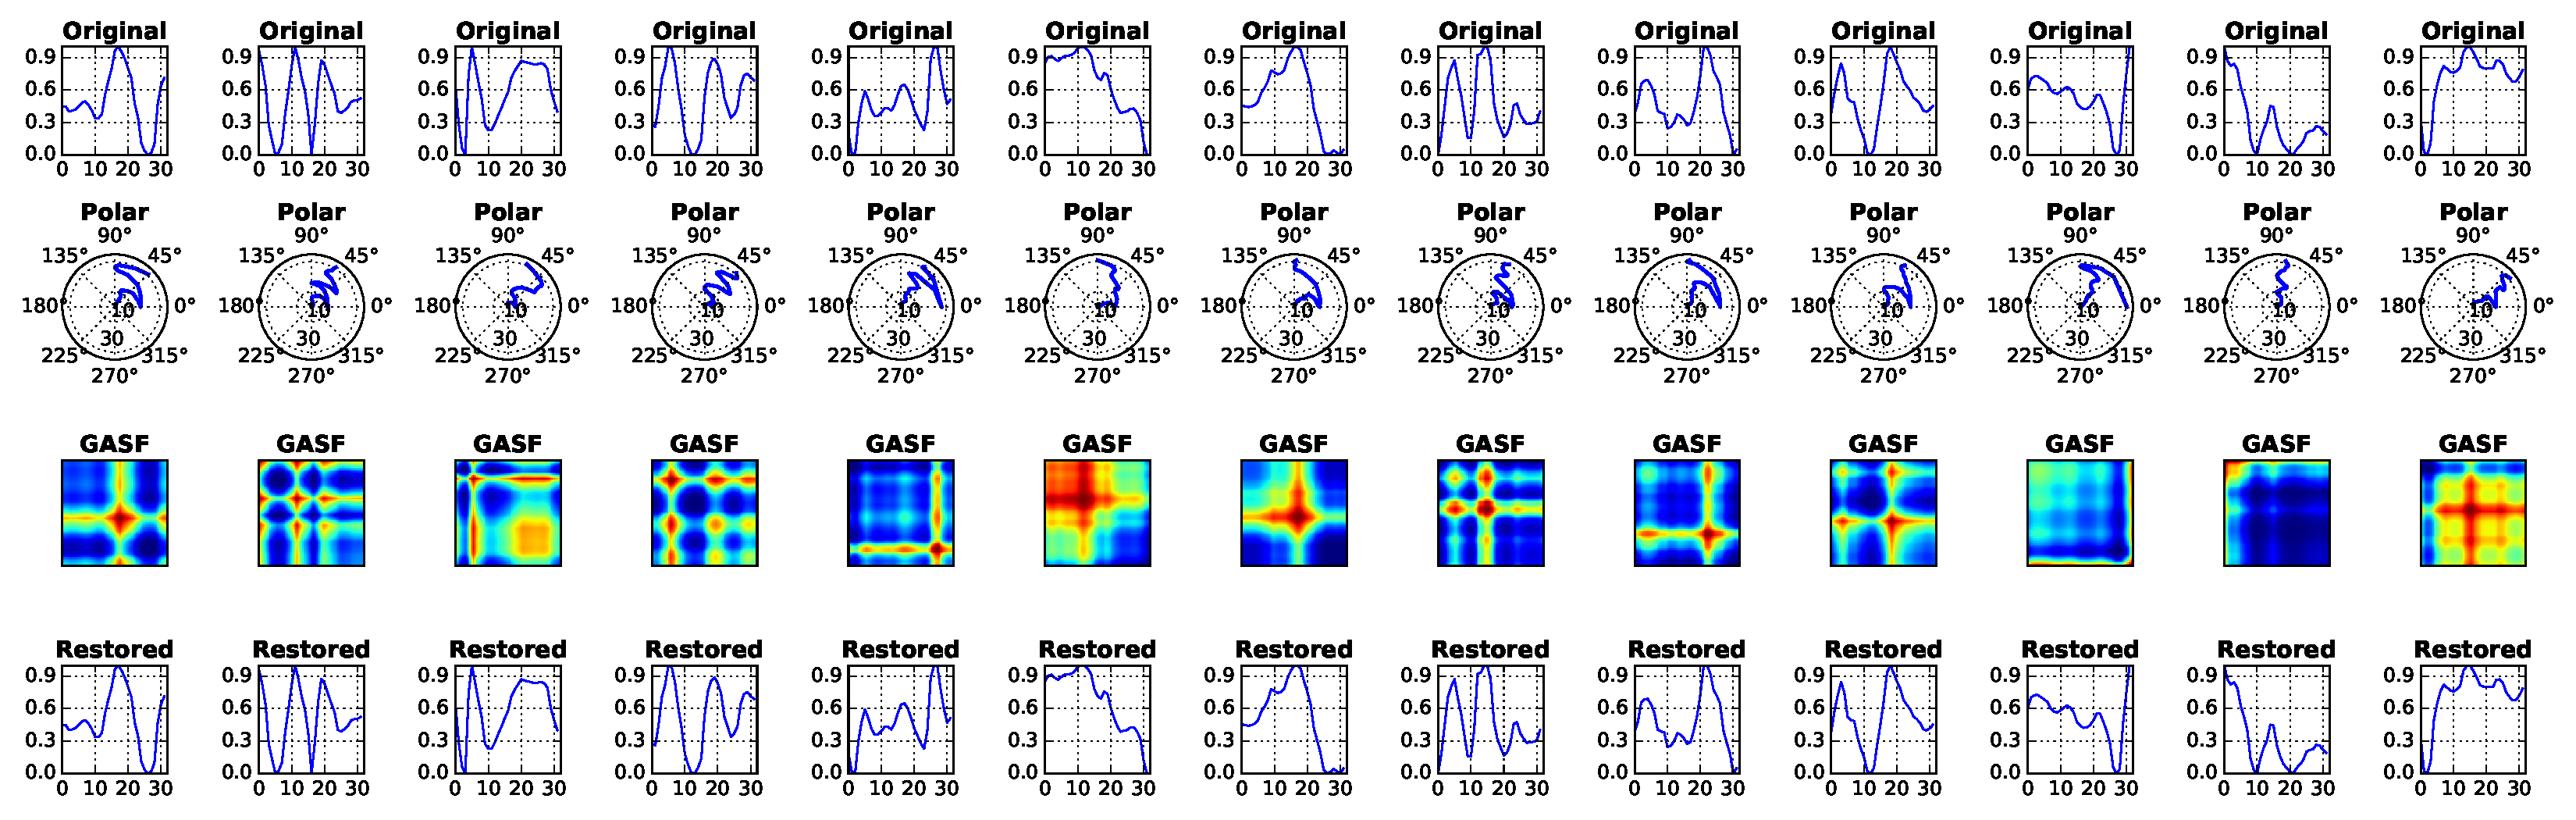
\includegraphics[width=\textwidth]{images/05-modeling/gasfpipeline.eps} 
 \caption{Conversion of time series into a~\gls{gasf} image and then back into its original space.}
 \label{figure:gasf_example}
\end{figure}

\subsubsection{Latent Dirichlet Allocation}
\glsdesc{lda} is one of the most simple and influential topic models. A topic model is a formal statistical relationship between a group of observed and latent (unknown) random variables, which specifies a probabilistic procedure to generate \textit{topics}~\citep{reed_latent_2012}. The \textit{topics} are defined as a probability distribution over a collection of words and can be seen as generating mechanisms for words in a documents. The idea behind the method is that of assuming a generative procedure from which several topics are likely to have generated the words. Each document then is represented by a vector of proportion describing to which proportion each topic are estimated to have contributed to the document, \ie the presence of words in it. Such vector is called the \textit{mixture proportions}.

\begin{figure}[H]
  \centering
  \begin{tikzpicture}
    [
      observed/.style={minimum size=15pt,circle,draw=blue!50,fill=blue!20},
      unobserved/.style={minimum size=15pt,circle,draw},
      hyper/.style={minimum size=1pt,circle,fill=black},
      post/.style={->,>=stealth',semithick},
    ]

    \node (w-j) [observed] at (0,0) {$w_{d,n}$};
    \node (z-j) [unobserved] at (-1.5,0) {$z_{d,n}$};
    \node (z-prior) [unobserved] at (-3,0) {$\theta_d$};
    \node (z-hyper) [label=above:$\alpha$] at (-4.5,0) {};
    \node (w-hyper) [unobserved] at (2,0) {$\beta_k$};
    \filldraw [black] (-4.5,0) circle (3pt);
    
    \node (eta-hyper) [label=above:$\eta$] at (3.5,0) {};
    \filldraw [black] (3.5, 0) circle (3pt);
    
    \path
    (z-j) edge [post] (w-j)
    
    (z-hyper) edge [post] (z-prior)
    (z-prior) edge [post] (z-j)

    (w-hyper) edge [post] (w-j)
    (eta-hyper) edge [post] (w-hyper)
    ;

    \node [draw,fit=(w-j) (z-prior), inner sep=14pt] (plate-context) {};
    \node [above right] at (plate-context.south west) {$D$};
    \node [draw,fit=(w-j) (z-j), inner sep=10pt] (plate-token) {};
    \node [above right] at (plate-token.south west) {$N$};
    \node [draw,fit=(w-hyper), inner sep=10pt] (plate-topic) {};
    \node [above right] at (plate-topic.south west) {$K$};
  \end{tikzpicture}
  \caption{LDA model diagram~\citep{blei_latent_2003}. In our context, each word $w_{d,n}$ corresponds to a window of data from the accelerometer attached to the player during play. In turn, a gameplay is interpreted as a document d (set of player generated words). $z_{d,n}$, represents the type (topic) assignment for a given word $w_{d,n}$ and $\theta_{d}$ is the mixture proportions representing the game session. In this work we are interested in representing the player game session by $\theta_{d}$.}
  \label{fig:graphical-model}
\end{figure}

For instance, consider a text document about governmental investments in sport stadiums. It can be assumed that it is a collection of words generated from different distributions (different topics) that take into account contexts like \textit{finance}, \textit{sports}, \textit{public administration} and \textit{life quality} improvements. In such discrete word distributions (over the same vocabulary) each word is weighted by its relationship to the context its is associated to. As an example, the word \textit{stadium} would have a higher likelihood under the topic about sports than under a one representing public administration or finance. Thus, each word, yet present in all topics, is weighted different according to their relationship in the document corpus. The~\glsdesc{lda} algorithm does not provide a meaning to the topics, but the programmer can attribute a meaning to it based on the words with higher probability.

The graphical model shown in Figure~\ref{fig:graphical-model} presents the basic structure of the~\gls{lda} model~\citep{blei_latent_2003}. For our purposes, as in~\cite{smith_mining_2016}, the \textit{K}-th probability distribution over input words $\beta_{k}$ (topic k) is representative of the $K$ groups (types) of player motion styles in which we are interested in. Each document $d$ corresponds to a game play session for the game and belongs to the corpus $D$ of all observed player sessions.

In these terms, a document may present multiple types $\beta_{k}$ with mixture proportions $\theta_{d}$. The mixture of proportions $\theta_{d}$, as explained above, defines a player at each instant of time by describe to what proportion each discovere topic contributes to the data generated in play session $d$. The choice of the $N_{D}$ words comes from $\overline{\beta}_{d}$, which acts as the weighted average of the game play types for a given document. This average is defined as follows~\citep{blei_latent_2003,smith_mining_2016}:

\begin{equation}
\overline{\beta}_{d} = \sum_{n=1}^{K} \theta_{d}(k) \cdot \beta_{k}
\end{equation}

The \textit{n}-th word $w_{d,n}$ of document \textit{d} is, in our case, the~\gls{gasf} encoding obtained, as we will explain later. $z_{d,n} \in \{1:K\}$ refers to the random motion type from which a word is drawn from and is an auxiliary variable that makes inference easier. Following the standard~\gls{lda} model, $\alpha$ and $\eta$ are hyperparameters that control the sparsity in the mixture proportions and word distributions~\citep{smith_mining_2016}.

\subsubsection{Autoencoder}\label{sec:autoencoder}

In many problems, we may have to deal with highly dimensional data that represent the situation of the world as captured by the sensors. Given that the raw data dimensionality could be practically intractable, the common procedure in these cases is to reduce the dimensionality possibly keeping only the important features of the input data.

In image processing, for instance, understanding which pieces of an image represent a significant aspect for the task ahead is not a trivial issue. Significance may be related to specific parts of the image and may depend on many aspects. A common technique to face this issue is autoencoder.
Autoencoder is an unsupervised learning technique that learns a representation of the input data, usually derived by means of non-linear transformations of the input~\citep{goodfellow_deep_2016}. A typical implementation of autoencoder consists of a feedforward neural network that first encodes the input into a code, the representation, and then reconstructs the input from it by means of a decoder (see Figure~\ref{fig:autoencoder_architecture}).

\begin{figure}[h]
\centering
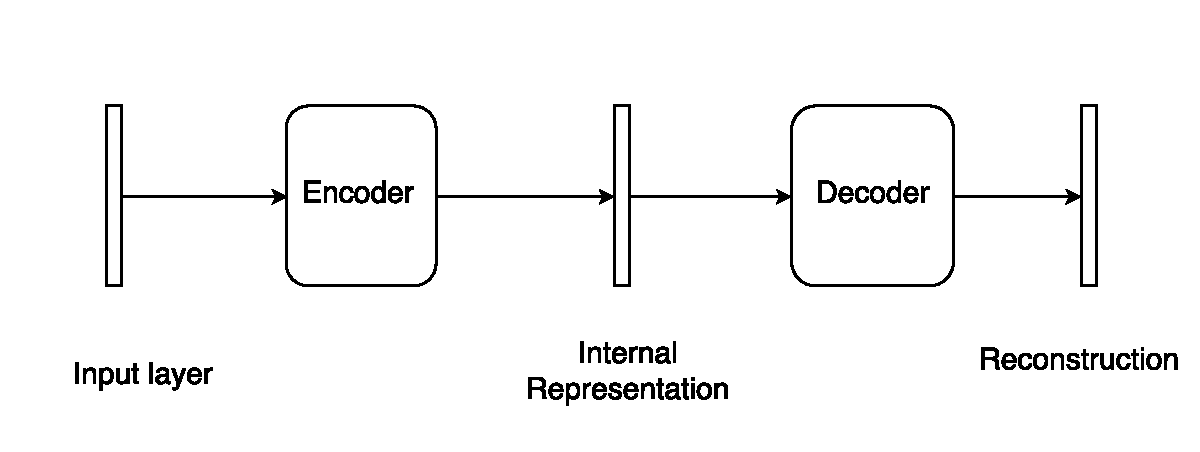
\includegraphics[width=.9\columnwidth]{images/05-modeling/autoencoder_architecture}
\caption{General architecture of an autoencoder; the input layer is processed by an encoder that transforms it. The derived representation is then decoded by a decoder that yields a reconstruction.}
\label{fig:autoencoder_architecture}
\end{figure}

In general, autoencoders are good at capturing the structure of the input and tend to represent it well~\cite{goodfellow_deep_2016}. We can understand an autoencoder as a neural network that tries to copy its input to its output. We can represent its general architecture with the following terminology:

\begin{itemize}[leftmargin=*,labelsep=5.8mm]
	\item the input $x$,
  \item the {encoder function}, $f(x)$, composed of some hidden layers,
  \item the {code}, or internal representation, of the input $h$,
  \item the {decoder function}, $g(x)$, composed of other hidden layers,
  \item the reconstruction obtained from the decoder, $r$.
\end{itemize}

A {loss function}, $L(x, r)$, should also be defined to evaluate how close the reconstruction is with respect to the input.
A simple loss function is shown as Equation \eqref{eq:loss_autoencoder}.

\begin{equation} \label{eq:loss_autoencoder}
L(x,r) = \sum_{i} (x_i - r_i)^2
\end{equation}

However, if we do not impose any restriction, the transformation it learns would be an identity, since this would perfectly reconstruct the input. To prevent this transformation, two approaches have been devised~\citep{goodfellow_deep_2016}. The first, called \textit{undercomplete autoencoder}, adopts a representation smaller than the input (see Figure \ref{fig:under_over_autoencoder}a), while the latter, \textit{overcomplete autoencoder}, uses a representation with a dimension larger than the input (see Figure~\ref{fig:under_over_autoencoder}b). Although increasing the representation size is counterintuitive in order to sparsely represent the input, this technique has proven its effectiveness.

\begin{figure}[h]
\centering
    \begin{subfigure}[h]{5cm}
        \centering
        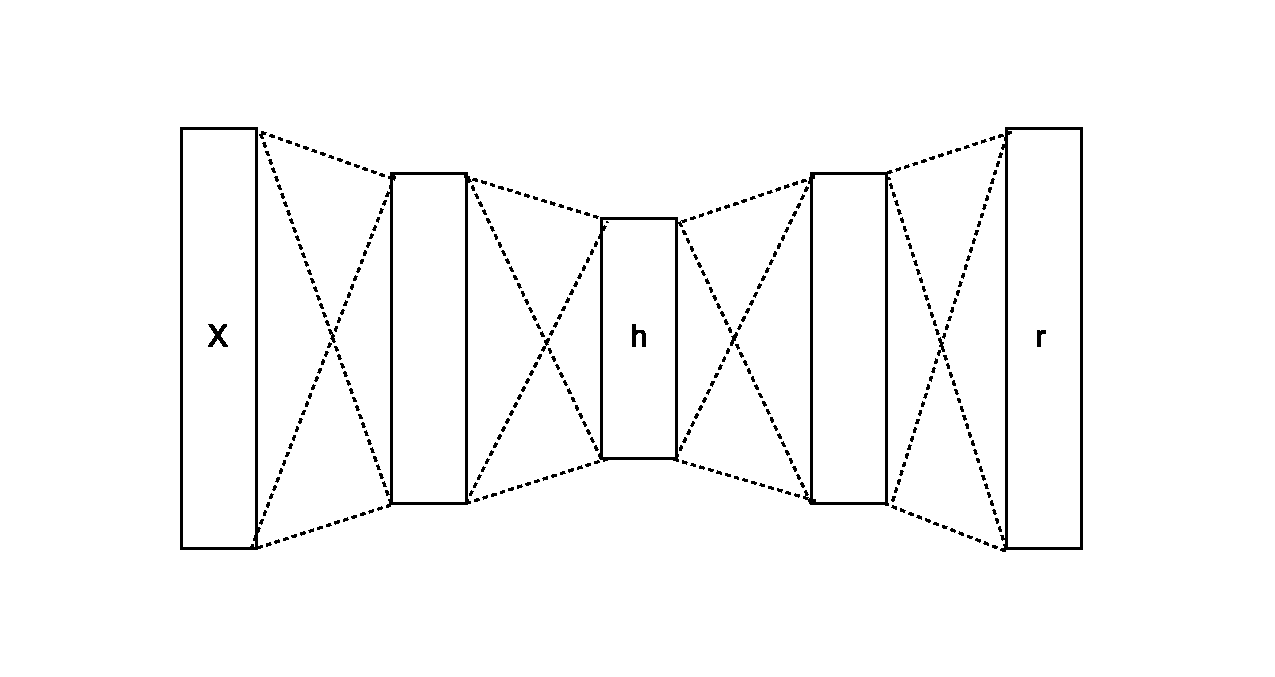
\includegraphics[width=4cm]{images/05-modeling/undercomplete_autoencoder}
        \caption{}
        \label{fig:undercomplete}
    \end{subfigure}
    ~
    \begin{subfigure}[h]{5cm}
        \centering
        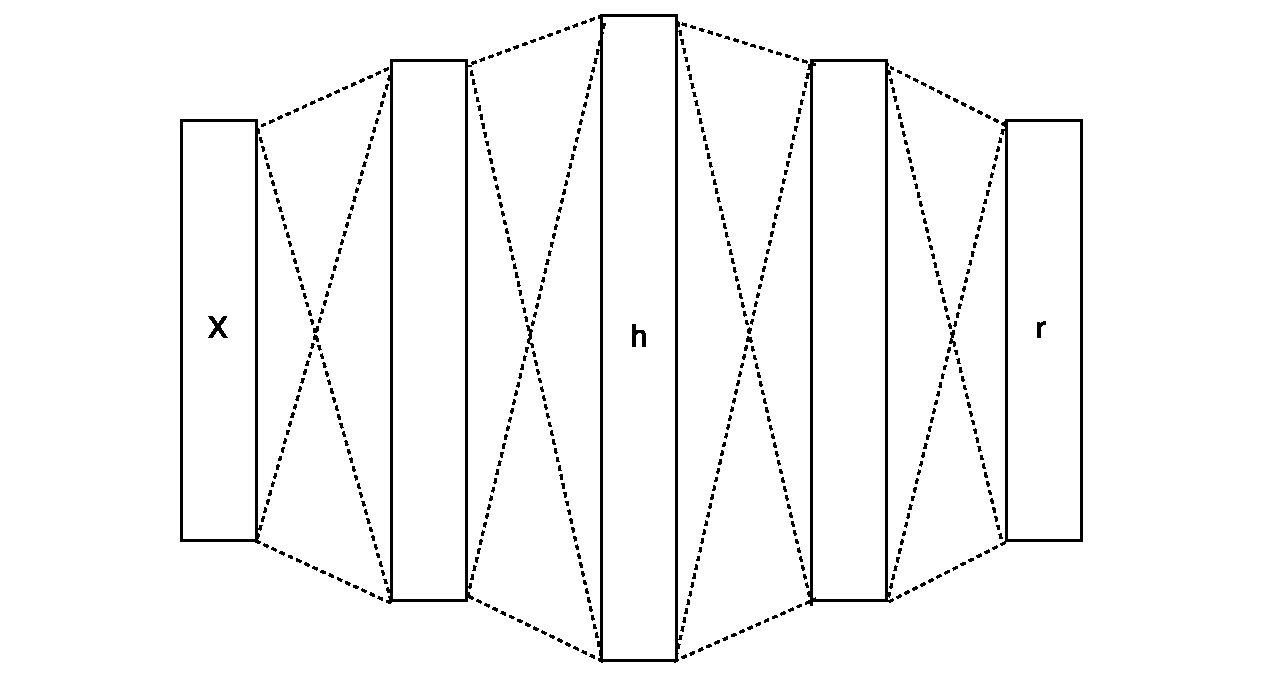
\includegraphics[width=4cm]{images/05-modeling/overcomplete_autoencoder}
        \caption{}
        \label{fig:overcomplete}
    \end{subfigure}  \vspace{-6pt}
    \caption{a) Representation of an undercomplete autoencoder, where the representation has a lower dimension with respect to the input. b) Representation of an overcomplete autoencoder, which uses a larger space to represent the input.}
    \label{fig:under_over_autoencoder}
\end{figure}

The undercomplete autoencoder is the oldest and best known architecture for the autoencoder and also the one we use in our work. The code the autoencoder derives is smaller than the input: it learns how to combine the input so that the relevant information is retained in a lower dimensional space. The combination is often non-linear due to a non-linear activation function of the neurons. On~the other hand, the decoder function learns how to unroll such compressed code in order to obtain an extended representation. This architecture could be trained using the classic back-propagation approach, although different methods are available~\citep{goodfellow_deep_2016}.

The overcomplete autoencoder, instead, increases the dimension of the representation; however, as already mentioned, the model could easily learn the identity transformation. In order to tackle this issue, the common approach is to apply a regularization term over the weights of the network. In general, a $l_1$ penalization is added to the loss function.
In this way, the representation will be sparse since some of the dimensions are set to zero.
However, this new architecture would be more complex to train since the model would be larger than the previous one, although still providing a sparse representation. Despite its sparsity, this architecture is able to extract more information from the input, and it is often used to capture also the input distribution and not just the structure of $x$. It is not possible to estimate such a distribution with an undercomplete autoencoder since such a task would require a higher representation capacity.

\begin{figure}[h]
    \centering
    \begin{tabular}{ccc}
        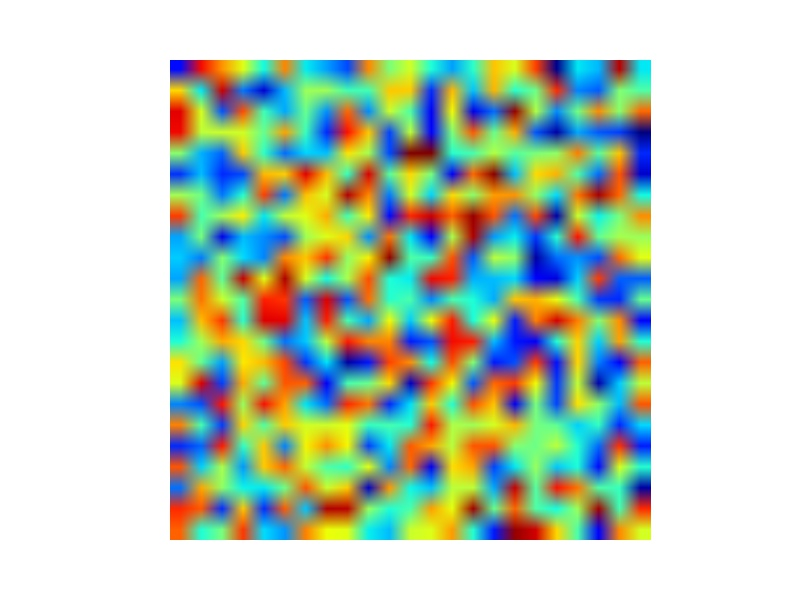
\includegraphics[width=0.2\columnwidth]{images/05-modeling/autoencoder_levels/autoencoders_2_0} &
        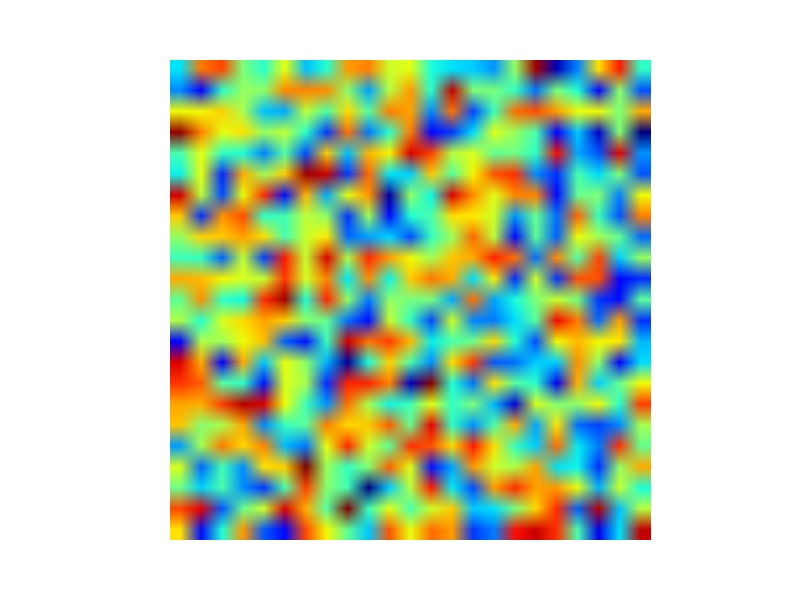
\includegraphics[width=0.2\columnwidth]{images/05-modeling/autoencoder_levels/autoencoders_2_1} &
        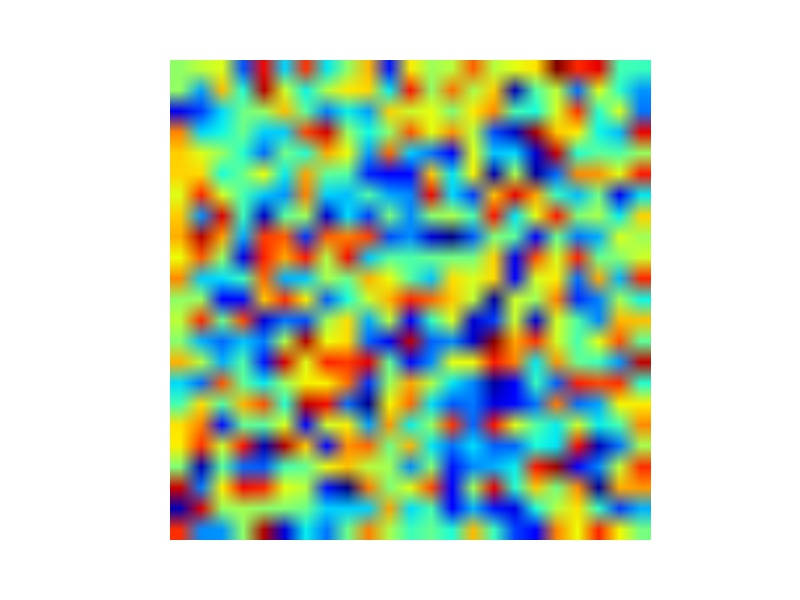
\includegraphics[width=0.2\columnwidth]{images/05-modeling/autoencoder_levels/autoencoders_2_2} \\
        (\textbf{a}) & (\textbf{b}) & (\textbf{c}) \\
        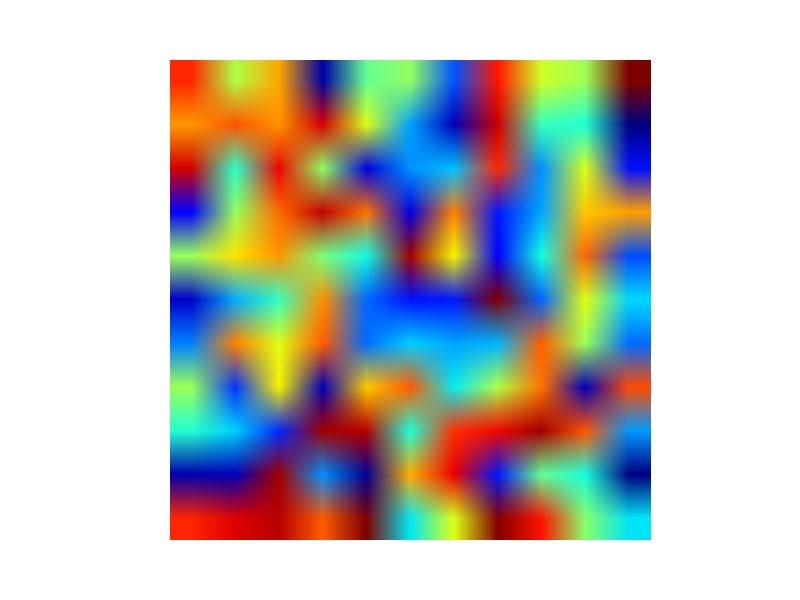
\includegraphics[width=0.2\columnwidth]{images/05-modeling/autoencoder_levels/autoencoders_4_0} &
        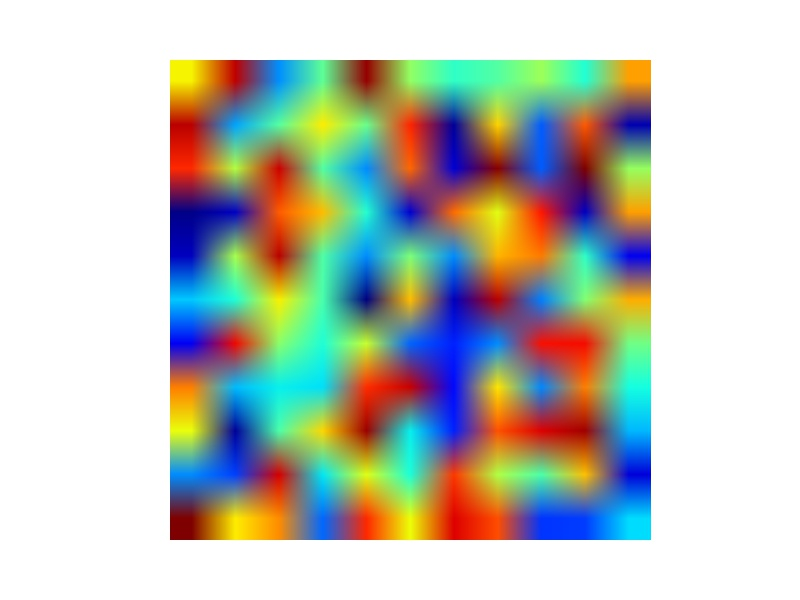
\includegraphics[width=0.2\columnwidth]{images/05-modeling/autoencoder_levels/autoencoders_4_1} &
        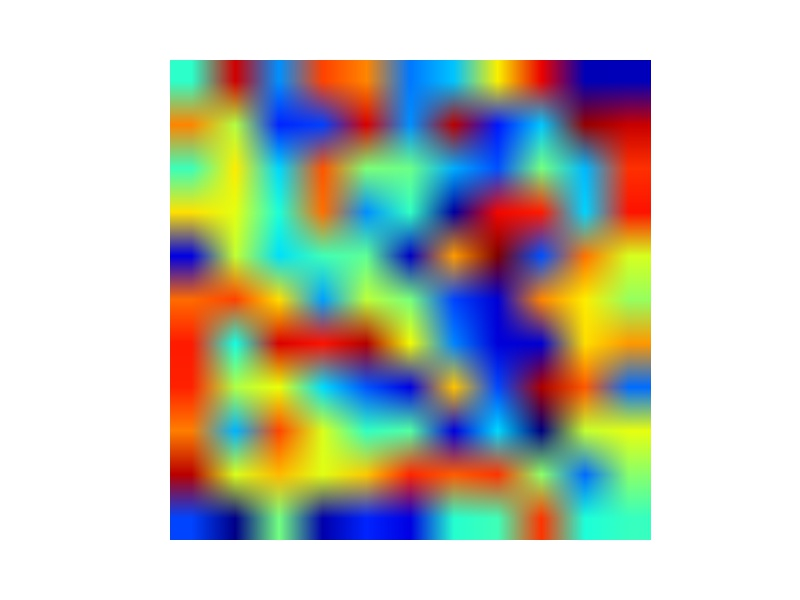
\includegraphics[width=0.2\columnwidth]{images/05-modeling/autoencoder_levels/autoencoders_4_2} \\
        (\textbf{d}) & (\textbf{e}) & (\textbf{f}) \\
        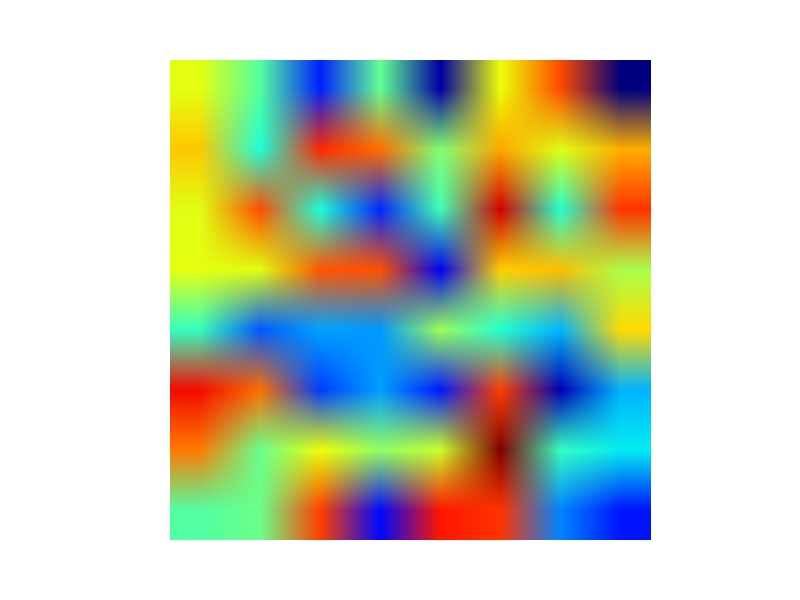
\includegraphics[width=0.2\columnwidth]{images/05-modeling/autoencoder_levels/autoencoders_7_0} &
        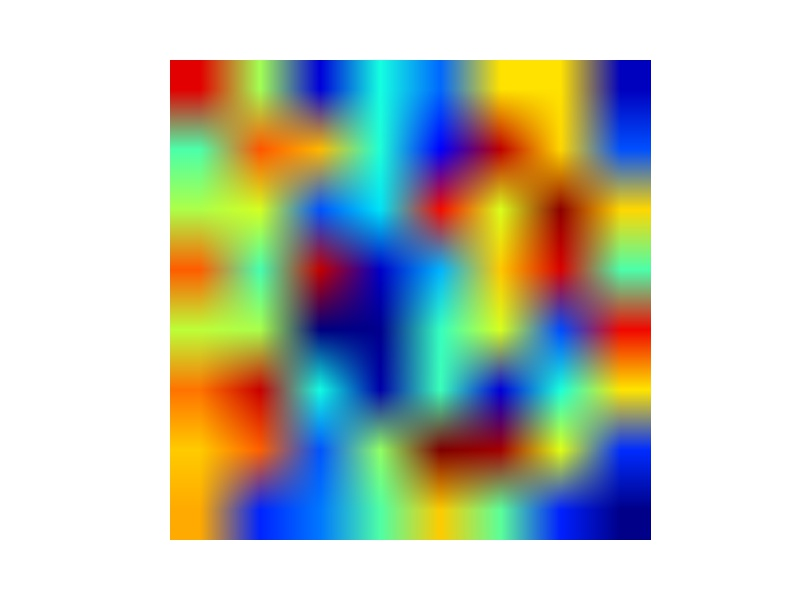
\includegraphics[width=0.2\columnwidth]{images/05-modeling/autoencoder_levels/autoencoders_7_1} &
        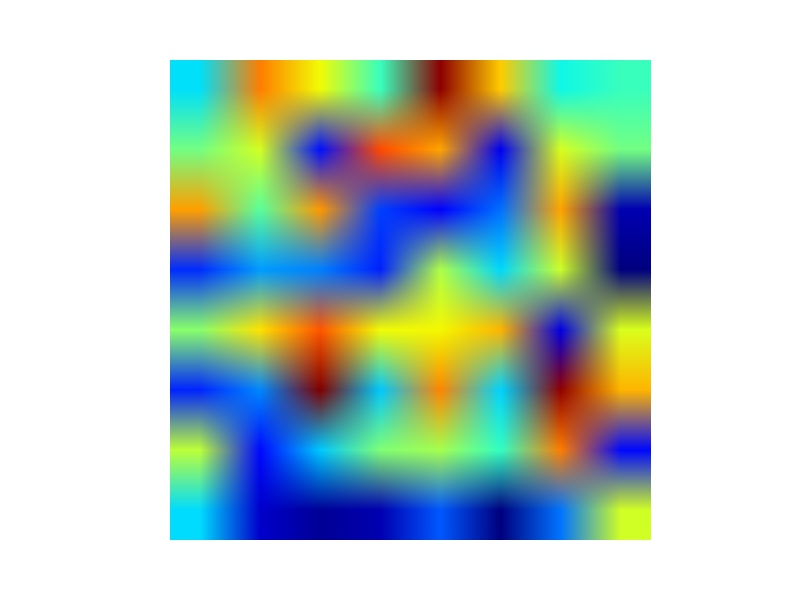
\includegraphics[width=0.2\columnwidth]{images/05-modeling/autoencoder_levels/autoencoders_7_2} \\
        (\textbf{g}) & (\textbf{h}) & (\textbf{i}) \\
    \end{tabular}
    \caption{Example layers from the trained autoencoder. (a--c) represent the information extracted by the first layer of the autoencoder. It is hard to grasp the meaning of the representation derived. Going deeper, in (d--f), the representation seems to become more clear and with a structure. Indeed going directly to the obtained code, in (g--i), we can see a more accentuate structure composed mainly of horizontal or vertical lines.}
    \label{fig:levels_autoencoder}
\end{figure}

In this work, we adopt an undercomplete autoencoder, since our goal is to represent an image in a lower dimensional space. 
Our architecture has multiple layers: the first layer takes only the input, while the following ones decrease in size with the power of two.
We represent the input with a code having 64 dimensions; thus, from an input of 1024 features, we derive a representation of 64 components using an autoencoder.

The reconstruction of the input by the decoder function has a very low loss, below 0.05\%. The~layers obtained by the encoder are often difficult to understand by people; for instance, in Figure~\ref{fig:levels_autoencoder}a--c, we can observe the first layer, and we cannot derive any structure or meaning from it. However, looking at deeper levels, the layers show a clear structure; in Figure~\ref{fig:levels_autoencoder}g--i, we can observe that the filters are extracting horizontal and vertical patterns. Indeed, most of the original images show a cross pattern, or multiple crosses; therefore, this representation seems to be able to represent the input data with a lower dimension.

\subsection{Modeling}
This section describes our approach to model the activity of the player, while emphasizing the differences and similarities with respect to existing methods. We take inspiration from approaches like~\cite{smith_mining_2016, wang_encoding_2015, wang_imaging_2015} and aim at modeling game sessions as ``documents'', where player's acceleration data are considered as ``words''. We use~\gls{lda}~\cite{blei_latent_2003} to categorize the player's motion profile as a composition or mixture of game play motion types, the latter being analogous to the ``topics'' in the general application of \gls{lda} for document modeling.

Differently from~\cite{smith_mining_2016}, our input word atoms are not discrete. Instead, they are continuous (acceleration data) and also are not attached to any explicit meaning. For instance, in \cite{smith_mining_2016} the natural interpretability of joystick input signals like ``left'' and ``right'' is available: the inputs convey their respective meaning when controlling a game character. In our case the raw accelerometer data carry no obvious absolute meaning from which a discrete tag can easily describe. In other words, in our scenario tagging is difficult.

The method adopted for selecting the input words is based on sliding windows (just as in~\cite{smith_mining_2016}), without overlap. This means we segment the entire accelerometer signal into subsets, called windows, so as to produce words. For all effects, as mentioned above, to the context of the application of~\gls{lda}, the \textit{document} produced by a given player is the whole raw acceleration during a game session and the \textit{words} of such document are the windows extract from the acceleration.

For the job, we have used~\gls{gasf} images instead of~\gls{gadf} because the mapping functions of the re-scaled time series in $[\,0,1]\,$ are bijections, which allows for precise reconstruction of the original time series~\citep{wang_imaging_2015}. The reconstruction takes advantage of the the main diagonal of the~\gls{gasf}s, i.e., $\{G_{ii}\} = \{\cos{2\phi_{i}}\}$, and is performed as reported in Equation~(\ref{equation:reconstruction})~\cite{wang_imaging_2015}:

\begin{equation}\label{equation:reconstruction}
    \cos(\phi)=\sqrt{\frac{G_{ii}+1}{2}} \qquad \phi \in [\,0,\frac{\pi}{2}]\,
\end{equation}

An example of signal decomposition into~\gls{gasf} images is shown in Figure~\ref{fig:acc_signal_gasfs}. The figure shows data of about 30 seconds of real game play from a three-axis accelerometer (48.8 Hz). It also displays thirty five~\gls{gasf} segments of a linear combination of the multidimensional time series. The combination collapses the signal into a one dimensional one and easy the transformation into~\gls{gasf}. For this case, each image comprises 0.65 seconds with 32 samples.

\begin{figure}[H]
    \centering
    \begin{subfigure}[h]{\textwidth}
        \centering
        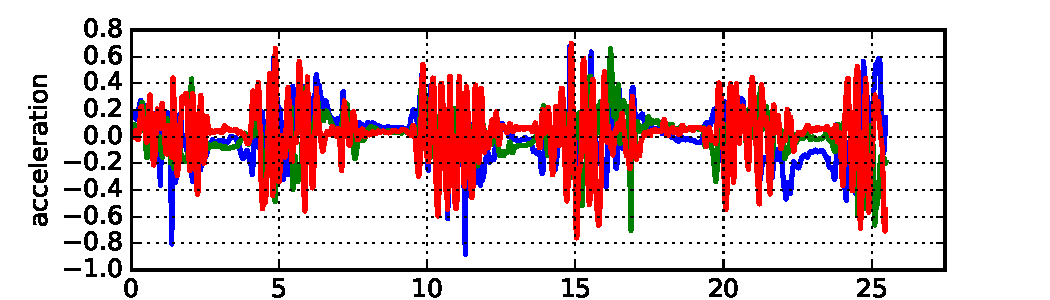
\includegraphics[width=0.9\textwidth]{images/05-modeling/example_signal.eps}
        \label{figure:accelerometer_signal}
        \caption{}
    \end{subfigure} \vspace{-6pt}
    ~
    \begin{subfigure}[h]{0.8\textwidth}
        \centering
        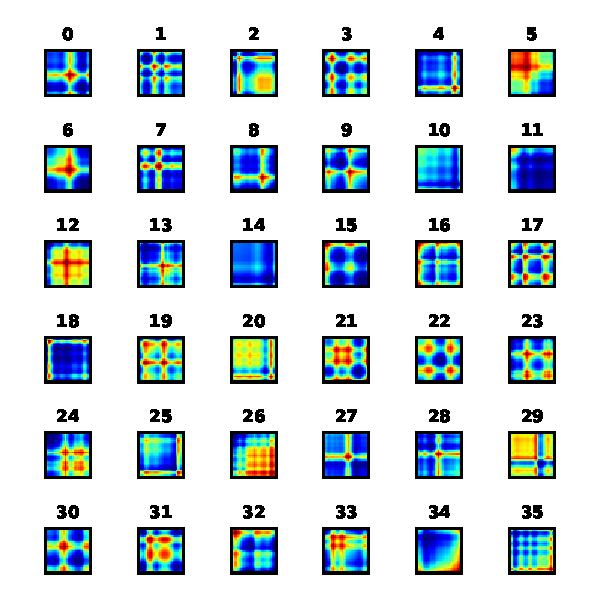
\includegraphics[width=0.8\textwidth]{images/05-modeling/example_gafs_seg.eps}
        \caption{}
    \end{subfigure} \vspace{-6pt}
    \caption{Example of the conversion of a time series into~\gls{gasf} images. a) Three-axis accelerometer data (48.8 Hz) of about 30 seconds of real game play. b) Thirty five~\gls{gasf} segments of a linear combination of the multidimensional time series. Each window comprises 0.65 seconds with 32 samples.}
    \label{fig:acc_signal_gasfs}
\end{figure}

Given recent advances in deep learning and pattern recognition for images, we take the route of~\citep{wang_encoding_2015} and exploit the applicability of autoencoders for extracting unsupervised features from~\gls{gasf} images (see Section~\ref{sec:autoencoder}). This is relevant since the process of feature engineering is time-consuming and laborious. Moreover, unsupervised feature extraction from such methods has been proven to work well~\citep{wang_imaging_2015, wang_time_2016}.
Sparse encoding via linear-algebra methods for dictionary learning is also a possibility. However, in our experiments, it turned out to be not as efficient as autoencoders. After encoding the images using an autoencoder we are left with a continuous description of each image and a procedure of discretization and dictionary learning for~\gls{lda} had to be performed. For this, we clustered the representations and used the so-obtained cluster centroids as dictionary words.We present details of our experimental activity in the next section. Our methodology is summarized in Figure~\ref{diagram:methodology}. In summary, 
for each available raw acceleration time series segments (windows) are extracted. Such segments are then turned into~\gls{gasf} images, whose representations (features) are obtained using an autoencoder. Since the basic \gls{lda} method works with a multinomial distribution of topics, hence a discrete distribution, we define a dictionary of visual words (through clustering) before inferring the~\gls{lda} variables. Therefore, for each~\gls{gasf} vector of representation we use its cluster centroid as a surrogate, allowing for the discretization into representative words. In the~\gls{lda} model, the latent variable of interest are the \textit{mixture proportions} and the \textit{topic} distributions, which basically estimate the participation of each uncovered topic (player types) in the generation of the player data.

\begin{figure}[h]
	\centering
    \begin{tikzpicture}[auto]
	\tikzstyle{b} = [rectangle, draw, fill=blue!20, node distance=0.5cm, text width=4em, text centered, rounded corners, minimum height=5em, thick]
    \tikzstyle{c} = [rectangle, draw, inner sep=0.2cm, dashed]
    \tikzstyle{l} = [draw, -latex',thick]
    
     \node [b] (time series) {Game time series};
     \node [b, right=of time series] (segments) {Segments};
     \node [b, right=of segments] (gasfs) {GASFs};
    	\node [b, right=of gasfs] (features) {GASFs features};
     \node [b, right=of features] (dict) {Dict. Learning};
     \node [b, right=of dict] (lda) {LDA};
    
     \path [l] (time series) -- (segments);
     \path [l] (segments) -- (gasfs);
     \path [l] (gasfs) -- (features);
     \path [l] (features) -- (dict);
     \path [l] (dict) -- (lda);
    \end{tikzpicture}
    \caption{The pipeline of our methodology.}
    \label{diagram:methodology}
\end{figure}

\subsection{Experimental Results}
In this section, we first report how to come up with the undercomplete representation for the~\gls{gasf} images using a simple autoencoder architecture, then we discuss how do we transform the extracted features into input words for the \gls{lda} model. Finally, we show the results when confronting the model output with human judgment. All experimental code used is available at the address ~\url{https://github.com/ewerlopes/lda-player-model.git}.

\subsubsection{Feature Extraction}
The first question we need to answer concerns the size of the windows used to segment the raw acceleration signal. This parameter regards the definition of the~\gls{gasf} images used as building blocks for the dictionary learning. The~window size should be large enough to capture motion patterns relevant for the player characterization, but not so large to confound their interpretation. We tried different window sizes and, similar to our previous experiments~\citep{oliveira_activity_2017}, decided to consider half a second of data per window without overlap, which allows for a quite fine-grained data representation.

We applied no preprocessing to the signal, since we were interested in observing how an autoencoder would perform using the unfiltered input. The expectation was that it would naturally compensate for the differences in the images, decisively choosing to capture important features (the main signal characteristic) and disregarding non-representative ones (the small associated noise). We defined an architecture composed by dropout and dense layers where only hyperbolic tangent activation functions where used, except in the last layer, where a linear activation function was used instead. The best performing architecture was composed by the following layers: dropout (0.1 drop fraction), dense (size = 256), dropout (0.2) and dense (size = 64). The same layers (in reversed order) were used for the decoder part. The decoder part is only used for accessing the quality of the representation, ~\ie in terms of the cost function define in section~\ref{sec:autoencoder} and is ignored once a good representation is acquired.

A window of half a second corresponds to 32 samples given our accelerometer average frequency of 48.8 Hz. As a consequence, we obtain images with a total of 1024 pixels. We did not applied~\gls{paa} for memory complexity reduction~\citep{wang_time_2016} since our computing environment was capable of handling the size of our representation well. Using the autoencoder, we manage to reduce the representation down to a 64-dimensional input, resulting in the reconstruction presented in Figure~\ref{fig:reconstruction}. The choice of a 64-dimensional representation is empirical, meaning that we were in principle searching for an undercomplete representation of the data and, upon testing with different configurations, we have chosen the one with the lowest reconstruction error. As it turned out, a 64-dimensional vector representation was the best result, given our dataset. 

\begin{figure}[h]
	\centering
	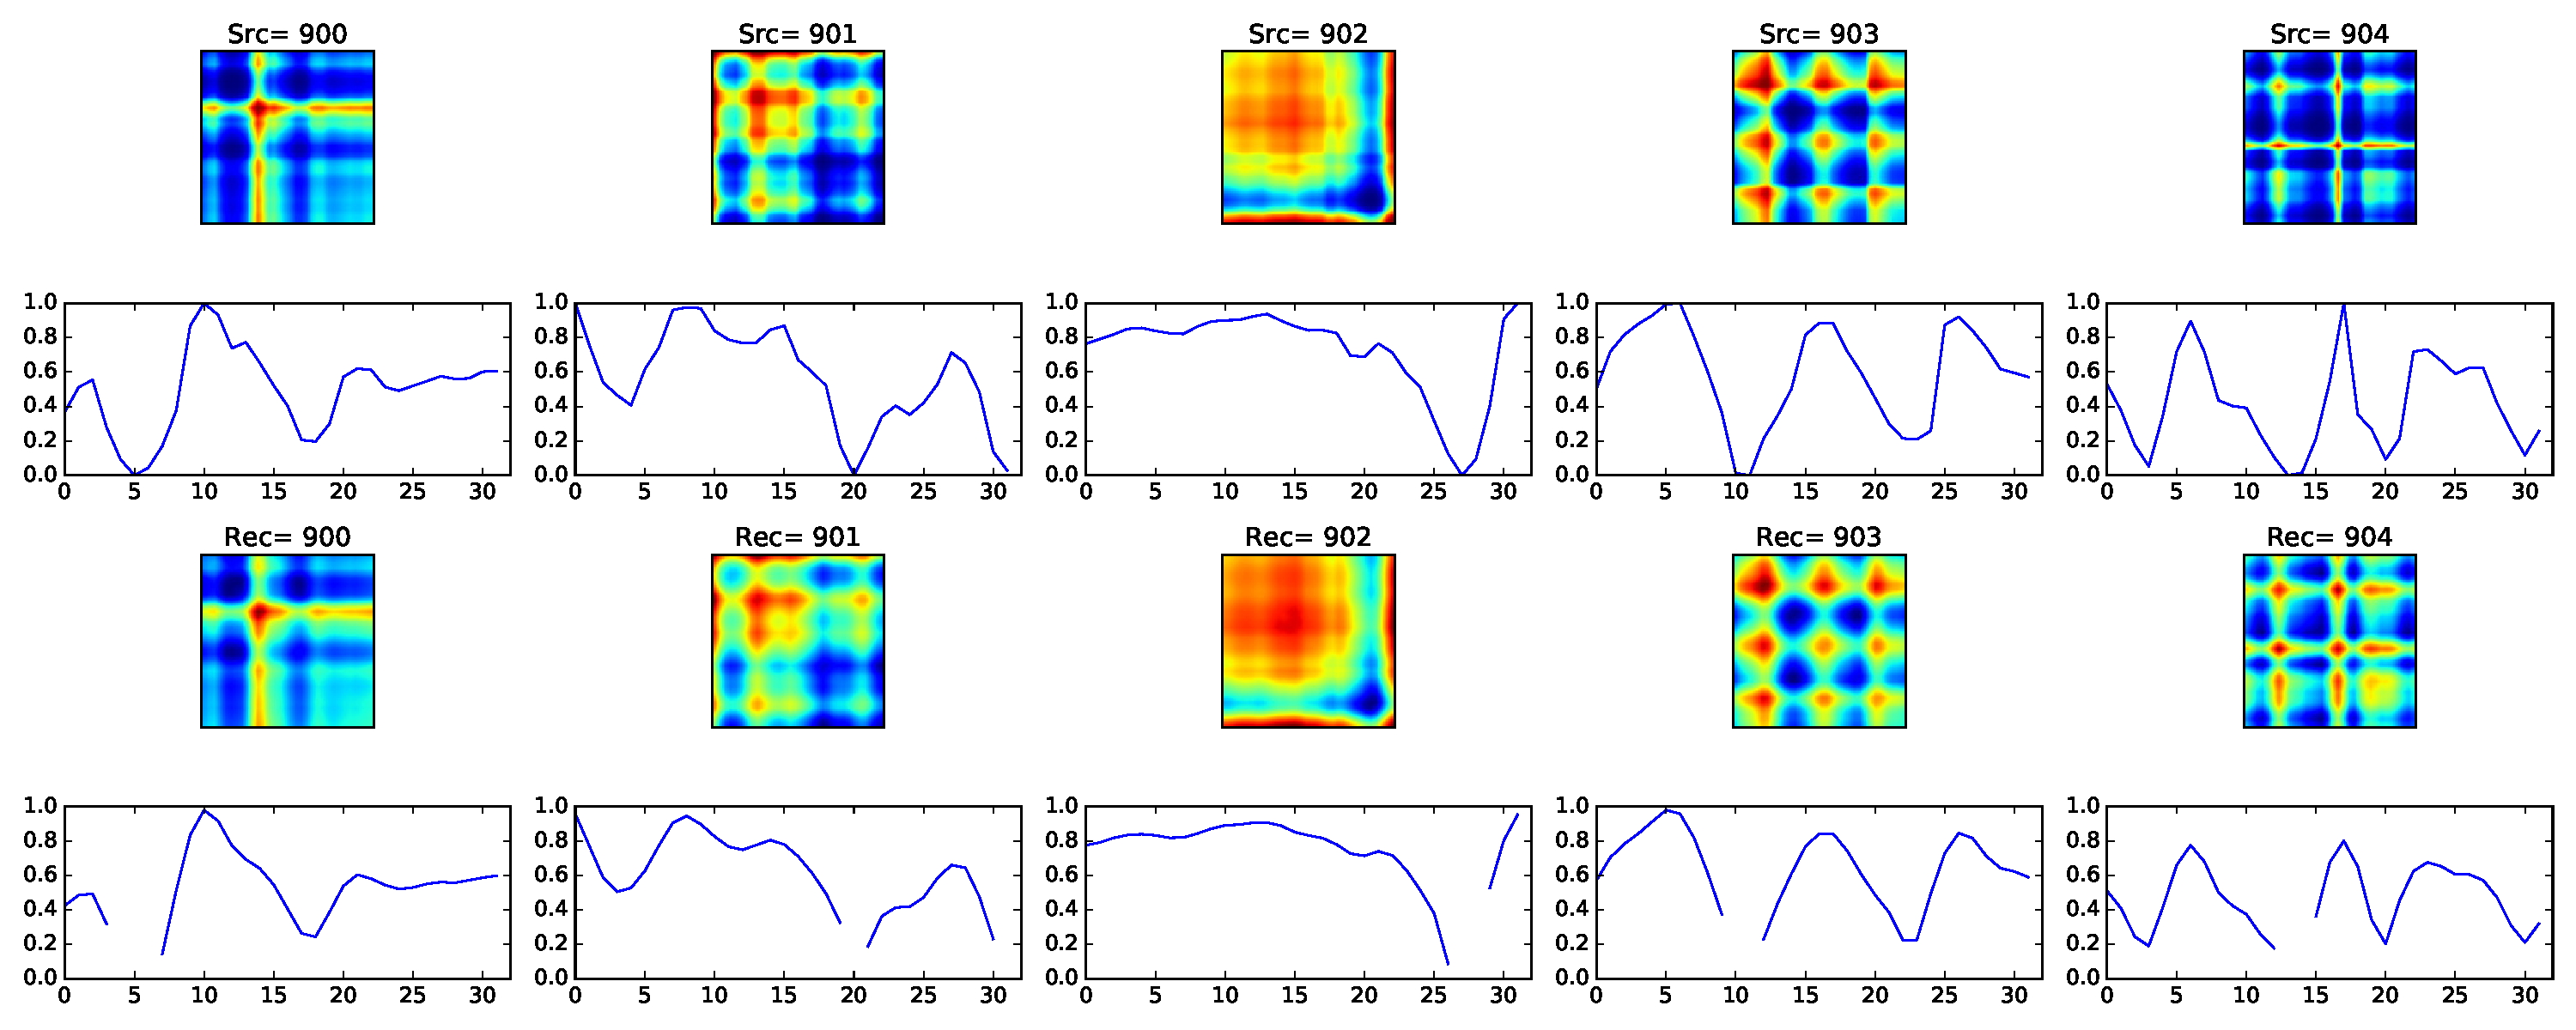
\includegraphics[width=\textwidth]{images/05-modeling/reconstructions.eps}
	\caption{Autoencoder reconstruction for five input segments corresponding to half a second of data (linear combination of the acceleration axis). ({Top line}) Input~\gls{gasf} images. ({Second line}) Original time series for each~\gls{gasf} input. ({Third line}) The autoencoder reconstruction for the input images. ({Forth line}) Time series from the reconstructed~\gls{gasf} images. Holes in the reconstruction are due to the error in the reconstruction of the images using the autoencoder.}
  \label{fig:reconstruction}
\end{figure}

It is possible to notice from the reconstruction result that, despite such a large compression (from 1024 to only 64 values), the input image relevant structure is captured. This can also be seen in the reconstructed time series. A closer look reveals that the autoencoder practically smoothed the time series while preserving the overall shape, this being a nice property that can help to prevent overfitting.

From Figure~\ref{fig:reconstruction}, we can also see that the obtained time series reconstruction presents some holes. This seems to be caused by the information loss in the reconstruction. In our experimentation, the data is well approximated and did not seem to affect the learning performance for the parameter of the~\gls{lda}. 

\subsubsection{Dictionary Learning and input word definition}
\glsdesc{lda} works by considering the relationship among word tokens with respect to a collection of documents. Therefore, in order to use the method, we needed to come up with a way to encode the diversity of~\gls{gasf} images into a discrete set of fixed tokens describing the motion primitives appearing in each game session. We opted to follow a similar approach to~\cite{prince_computer_2012} and further encode each extracted vector of feature as \textit{visual words}, finally composing the game session document. 

Here is how we proceeded: after getting the 64-dimensional vector representation for each~\gls{gasf} image, we cluster them into $V$ groups using the K-means algorithm. In this way, we define a dictionary of size $V$, with each word corresponding to a cluster centroid. Each game session is then translated into a collection of $V$ possible clusters, which can then be fed into the \gls{lda} algorithm.

From text mining and information retrieval, we know that having documents with different sizes can lead to some issues. In special, when using he bag of words assumption, \ie when not considering the ordering of words, as does~\gls{lda}, a small document may be included as in a larger one. This can lead to accuracy problems and misleading interpretation of performance. Additionally, in our scenario, it is problematic to have to evaluate long play session given that multiple interpretation about the player behavior can be assigned to the same session depending on the evaluator. Such ambiguity can definitely worsen the estimation of the model parameters.

In text mining, this issue is handled by imposing a weight based on the length of the document; in our case, instead, we decided to split each session into smaller segments of 15 s each. In this setting, the evaluation is more consistent, and it is possible that the behavior of a player will be maintained within segments. We decided this length for each document both for convenience with respect to the window length and from the empirical assumption that in each fraction of 15 seconds, the player can show a consistent behavior and that it can be somehow easily identifiable. In the next section, we present the results achieved.

\subsection{Validation}

Our ultimate objective is to represent the player motion style by a mixture of topic proportions following the \gls{lda} framework. The method by itself demands the programmer to initialize the desired number of topics. Thus, we had to perform a search for the optimal value for our dataset.

By performing grid search, we selected a range of values for the two main hyperparameters, namely dictionary size, for the input word definition, and number of topics. We would like to keep the number of topics low, preferably less than 10, since by observing our dataset, it is not possible to distinguish many groups of different motion styles; this suggests that a coarse-grained definition would be better. Choosing the number of topics to be at most 10, as in~\cite{smith_mining_2016}, the evaluation of the uncovered topics remains manageable, while maintaining a certain degree of freedom for the existing motion diversity.

The distribution of cluster centroids (words) given topics (our player motion types) is shown in Figure~\ref{fig:overall_game}.
Each line represents a topic, while each column represents a word. As one can see, there are no topics represented by the same distribution over the same word. Figure \ref{fig:overall_game} shows how much each word is important for the specific topic.

\begin{figure}[h]
    % TODO: fix the typo in the xlabel.
	\centering
	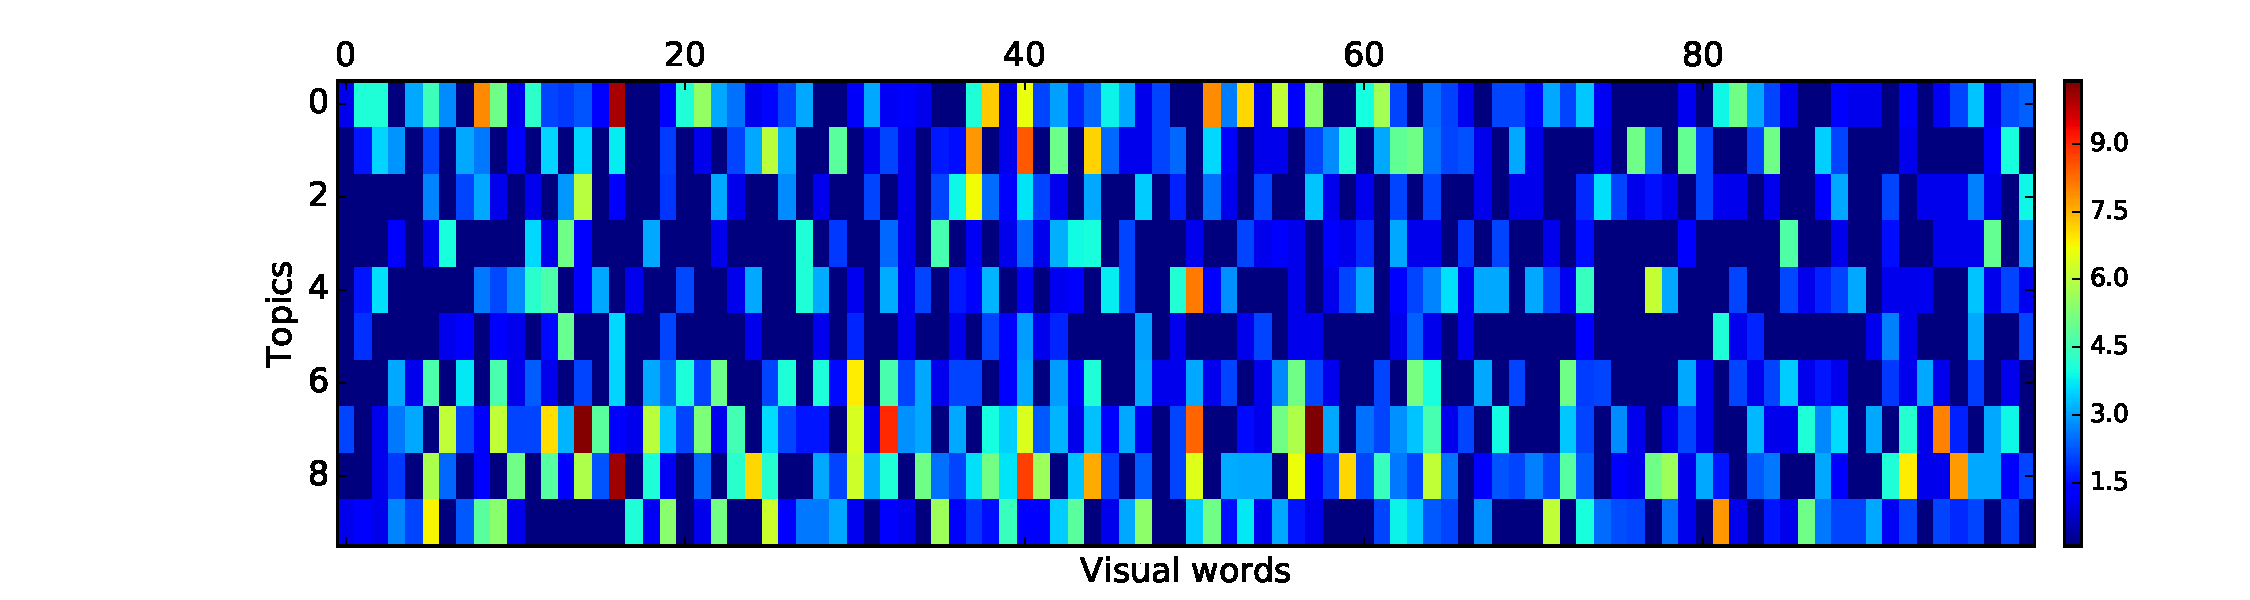
\includegraphics[width=\textwidth]{images/05-modeling/lda_heatmap.eps}
	\caption{Schematic representation of the game: each line represents a topic, while each column represents a word that is representative of the specific topic.}
  \label{fig:overall_game}
\end{figure}

In order to validate the discovered topics, we use human judgment. We invited volunteers to watch a set of pairs of recorded game segments (15 s each) and point out the similarities between players in their motivation as perceived by their motion. Subjects had to judge how similar, on a scale from 0--5, the movements of two players were. With this, we generated a similarity matrix to be used as the ground truth and main guide for deciding which hyper-parameter value to use and to check whether the proposed method could achieve reasonable results.

The similarity matrix was composed of $406$ independent evaluations from six different human subjects. The generated evaluation matrix was then compared with a cosine similarity matrix generated after training the \gls{lda} in our dataset. The similarity, in this case, is based on the mixture proportions among the discovered topics. 

We used this information to define the number of topics and the number of words. The best set of parameters is the one that presents a higher similarity compared to the one expressing human judgment, thus the smallest Mean Squared Error (MSE). The graph in Figure~\ref{hyperparameter_results} shows the results obtained varying the size of the dictionary (number of cluster centroids) and the number or topics. From it, we have decided to pick 100 as the number of visual words and 10 for the topics present in our dataset.

\begin{figure}[h]
	\centering
	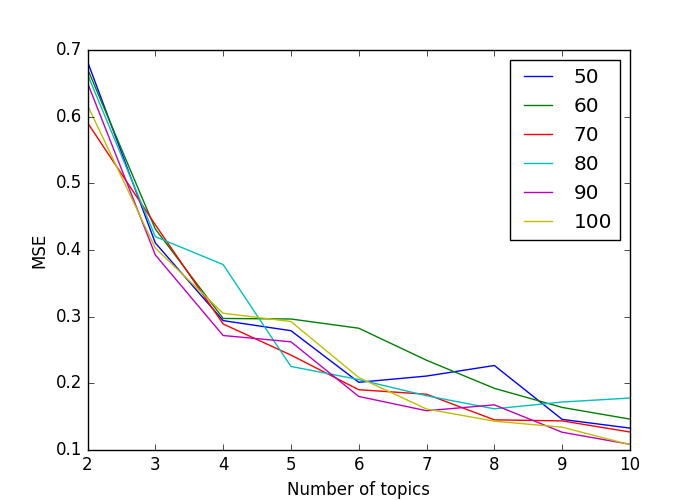
\includegraphics[scale=0.6]{images/05-modeling/mse_dictsize-50_100_10.png}
	\caption{The figure shows the hyperparameter tuning results. The~\gls{mse} is estimated with respect to the similarity expressed in the matrix containing the human judgment. The different lines represent the~\gls{mse} obtained for different dictionary sizes and number of topics.}
  \label{hyperparameter_results}
\end{figure}

The observed similarity results were verified by visual inspection of video logs from estimated similar players; that is, by checking how reported mixture proportions actually look similar in video. However, we state that much work should still be performed towards easily and reliably assessing model correctness and selection. This also relates to the possibility of confidently giving names to discovered motion types, very much in the way as is done in classic \gls{lda} for text categorization.

Another aspect that demands further investigation is how to avoid the decrease in accuracy when considering variable-sized game sessions. As mentioned before, game sessions with different sizes may artificially increase similarity in case one is a subset of another. The solution to this problem provides only a baseline, and much more sophisticated approaches to the problem should be~devised.

We believe that a potential way for improvements in interpretability and accuracy is that of removing the vector quantization in defining each topic. It would be interesting to remain in the continuous domain defined by our input data representation (GASF features), instead of relying on a fixed predefined vocabulary set used for training the \gls{lda}. Such vectorization is known to lead to information loss~\cite{hu_latent_2012}. To avoid such an issue, one possibility may be replacing the topic multinomial distribution by a mixture of continuous distributions such as Gaussians. This is akin to consider a word as a multidimensional point generated from the continuous mixture. Regarding this, we ackownledge the work of~\cite{hu_latent_2012} in which the authors propose the use of a continuous admixture model, named Gaussian-LDA, as an alternative to model a corpus of audio data. 

\subsection{Discussion}
The main advantage in using this approach, that can be used for clustering players into coherent groups based on the activity level, is that by using a autoencoder for representing the obtained~\gls{gasf}s the workload necessary for hand-crafting features is reduced. Also, one may play with other methods for image classification  as well as explore results from other clustering methods.

% The primary concern shown in~\cite{smith_mining_2016} is that of encoding user controller inputs into discrete tokens (words), allowing for the unsupervised identification of types of gameplay fostered by a particular game level.

% Unfortunately, such approach poses some challenges, as reported by the authors:
% \begin{inparaenum}
%   \item the difficulty in finding the associated relationship between controller inputs and gameplay types; as well as  
%   \item the difficulty to objectively define the gameplay types comprising their presence in different parts of the game.
% \end{inparaenum}

A probabilistic graphical model, such as~\gls{lda}, offers the possibility to capture players' style as a composition of multiple existing player profiles, which makes the model robust in capturing the high diversity of acceleration signals in our scenario. The basic assumptions are~\citep{smith_mining_2016}:

\begin{enumerate}[label=\Alph*.]
\item The ``input words'' (gameplay types, in our case) are assumed to occur in a document (session play-through) and describe a game session, allowing the categorization of types of gameplay;
\item A game setting (level, or in our case robot parameters related to difficulty) is assumed to foster and be represented as a mixture of several gameplay types;
\item Similar gameplay types can co-occur;
\item Similar players tend to produce similar gameplay types.
\end{enumerate}

While being able to quantify the extent to which each gameplay type is present in a game level, the related approach in~\cite{smith_mining_2016} has several limitations that prevent its direct use in~\gls{pirg}s, including:

\begin{enumerate}[label=\Roman*.]
    \item In a~\gls{pirg} game, like RoboTower v2, the human player is not likely to use controller inputs and, therefore, the structured information present in controller inputs is not well-defined;
    \item In~\gls{pirg}s, we often have a continuous stream of data coming from multi-channel sources %and we would like to have an on-line processing instead than a batch analysis of texts;
    \item In~\gls{pirg}s the difficulty to assign semantic meaning to some of the discovered gameplay types is high, since the source of information is a time series of data (e.g., player's quantity of motion, physiological signals), rather than controller inputs such as ``move left'', ``move right'', ``jump'', etc.;
    %\item The model inclusion of additional factors that affect the player's play style, such as in-game events or player skill attributes, is necessary.
\end{enumerate}

Our approach addresses the problem in the points I and II by giving means to process the continuous data available. In fact, the use of~\gls{gaf} images can be further exploited in multi-channel sources by putting together different sources in the same image similar to what it done in standard RGB image -- one color for each channel. 


\section{Considerations}
In this chapter we have proposed some ideas for player modeling in~\gls{pirg}s. The main contribution stems from the use of popular~\gls{ml} algorithms, such as~\gls{lda}, K-means and autoencoder to evaluate phenomena in our game scenario. The results show the capacity of the model in approximating the human evaluation as to what concerns the similarity among players. Further investigation can address strategies for increasing interpretability of the uncovered topics in the sense of whether each topic can confidently be associated with meaningful tags (\eg ``over excited'', ''lazy'', etc) similar to the ones given when using~\gls{lda} to text mining. We hope the experimentation detailed in this chapter will inspire further research and help to increase interest  in the design of~\gls{pirg}s.
